	\section{Overall Description}
		\subsection{Product Perspective}
		Ticket Tonight is a follow-on member of Ticketmaster’s mobile app for ticket sales. It relies on Ticketmaster‘s user database to provide users’ preference for event choice and previous activity records, along with events information such as event data, type, location, and ticket price to generate recommendation choices for users to choose. Then it leads the user to Ticketmaster’s own purchase system for ticket buying.
		\begin{center}
			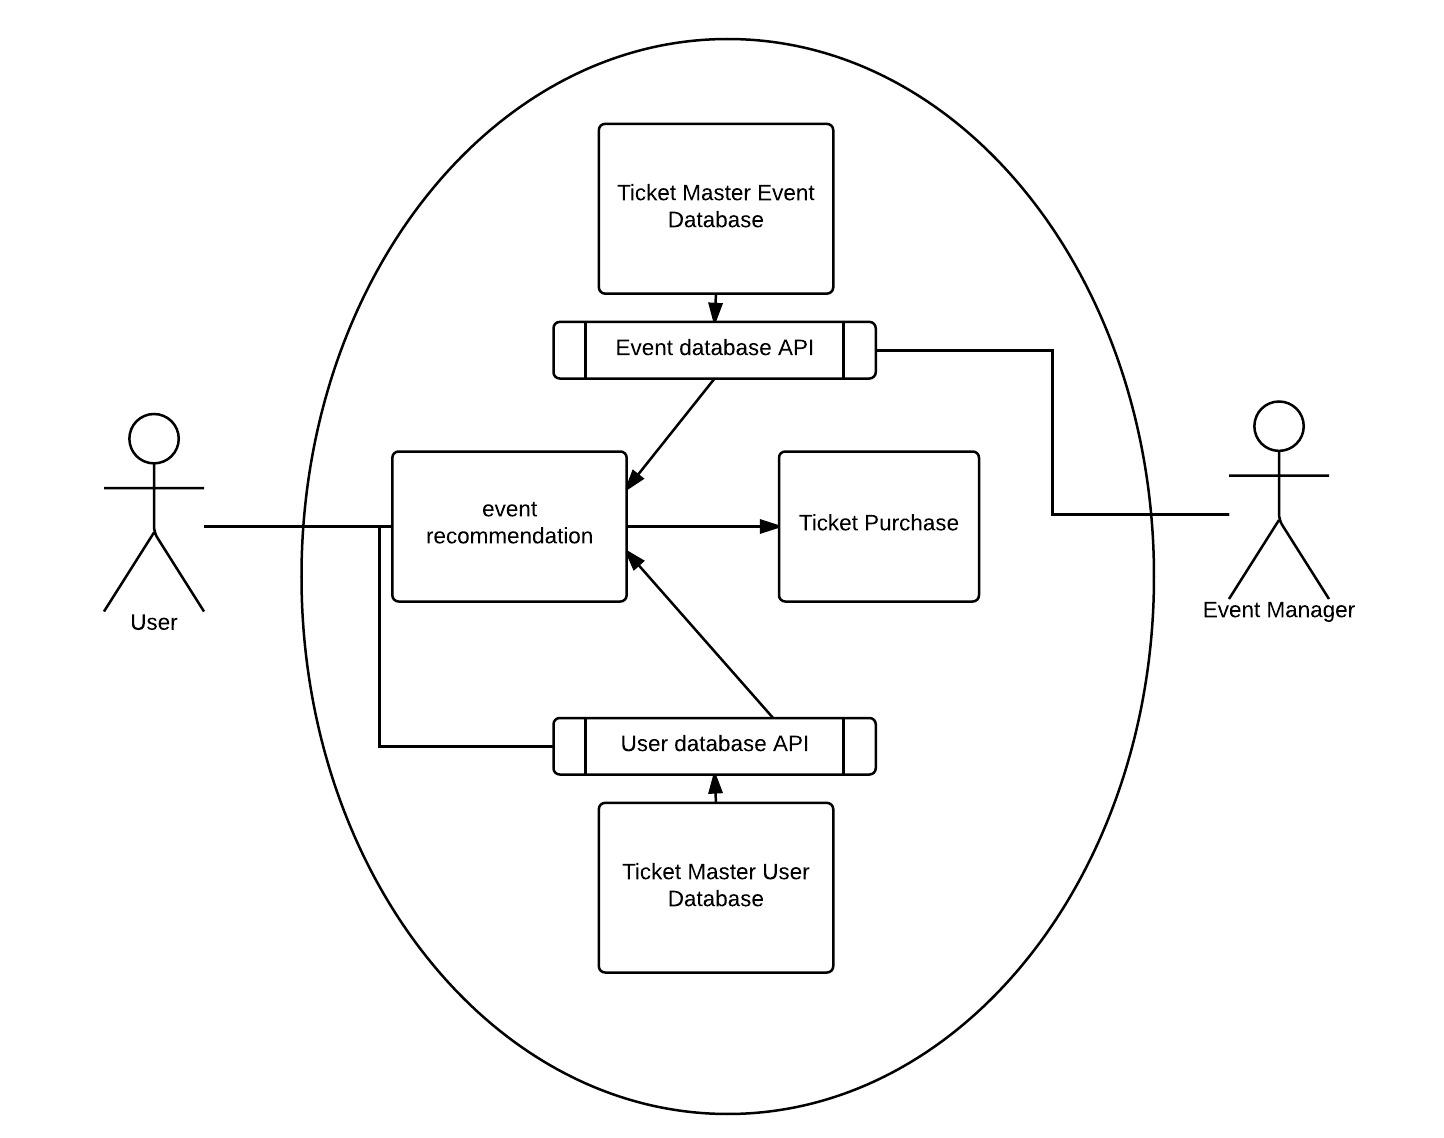
\includegraphics[width=90mm]{./pp1.jpg}
		\end{center}
		\subsection{User Classes and Characteristics}
		 There will be two main types of user classes for this app: event promoters and potential ticket buyers. Event promoters will be able to easily tell Ticketmaster of last-minute ticket availabilities through the app. The promoter can specify the number of tickets available and the price they’d like to set for those available tickets. Potential ticket buyers, which will be the majority of users, will be notified when an event would be a good match for them based on their Ticketmaster purchase history and preferences. Potential ticket buyers will be able to browse nearby events and filter the results by location and event type. 
		 \subsection{Operating Environment}
		 Initially, the Tickets Tonight app will be built for Apple’s iOS 8 mobile operating system, but will be supported on devices with Apple’s iOS 7.0 and later. It will support all devices running iOS 8, including the new iPhone 6, iPhone 6 Plus, iPad Air 2, and iPad mini 3.  The app will take advantage of these new display sizes and utilize the device’s location and TouchID sensors for a better user experience in receiving recommendations and completing ticket purchases. Given enough market demand, an Android version of the app will be developed. 